%!TEX root = ../thesis.tex
\section{平行グリッパの設計}
本研究では,リニアガイドとラック&ピニオン機構を用いた平行グリッパを設計した.図\ref{fig:hand}は平行グリッパの分解図である.グリッパの開閉には,QDDモータ(Steadywin GIM3505-8)を使用し,モータに取り付けたギアを介してラック&ピニオン機構で駆動する.グリッパのスライド部分にはリニアガイドを採用している.また,黄色の部品は3Dプリンタでの製作を行う.
\begin{figure}[htbp]
  \centering
  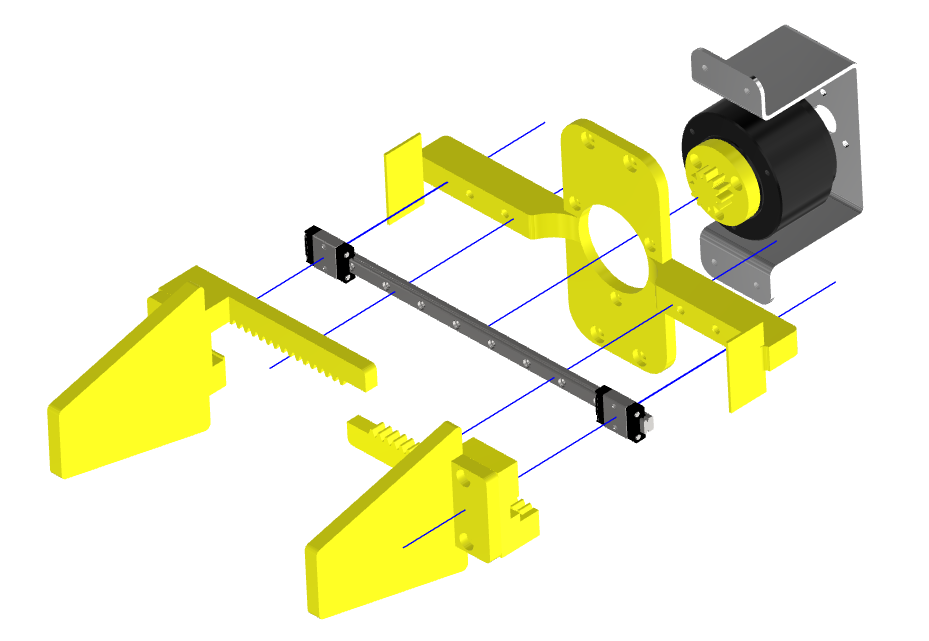
\includegraphics[width=10cm]{images/design/hand.png}
  \caption{Exploded view of parallel gripper}
  \label{fig:hand}
\end{figure}

\newpage